\documentclass[10pt,a4paper,notitlepage,twocolumn]{article}
\usepackage[margin=0.31in,footskip=0.25in]{geometry}
\usepackage{xpatch}
\usepackage[ngerman,english]{babel}
\usepackage[T1]{fontenc}
\usepackage[utf8]{inputenc}
\usepackage{amsmath,url,stackengine}
\usepackage{mathtools}
\usepackage{multicol}
\DeclareMathOperator{\Hessian}{Hess}
\usepackage{enumitem}
\usepackage{booktabs}
\usepackage{array}
\usepackage{derivative}
\usepackage{algorithm}
\usepackage{algpseudocode}
\usepackage{esvect}
\usepackage{amsfonts}
\usepackage{tikz}
\usetikzlibrary{shapes.geometric}
\usepackage{graphicx}
\usepackage[%  
    colorlinks=true,
    pdfborder={0 0 0},
    linkcolor=red
]{hyperref}
\usepackage{subcaption}
\usepackage{float}
\usepackage{amsmath}
\usepackage{stmaryrd}
%svg
\usepackage{svg}

\title{OPT202 Project 1: An articulated chain}
\author{Tatiana Naomi Yamamoto Silva, Yanyu Zhou}

\begin{document}
\maketitle
\section{Introduction}
This project explores the application of Newton's method for finding the static equilibrium of a chain composed of rigid bars in two-dimensional space. The problem is formulated as an optimization problem, with the constraints initially expressed as equalities. This formulation allows us to apply Newton's method to find the root of the non-linear system of equations, which in turn provides the desired static equilibrium. In the second part we transfer the constraints into inequalities in order to take advantage of convexity. By employing semi-definitive programming, we are able to efficiently solve the optimization problem.

\section{Part I: Newton's method}
\subsection{Setting up}
The problem is modelled as an optimization problem as below:
\begin{equation}\label{P0}
\tag{$P_{0}$}
\underset{\substack{x \in \mathbb{R}^n,\ y \in \mathbb{R}^n}}{\min} \ E(x,y) \quad \text{s.t. } c_i(x,y) = 0,\ i \in [1,...,N+1],
\end{equation}
where
$E(x,y) = \sum\limits_{i=1}^{N+1} l_i(x,y)\frac{y_{i-1}+y_i}{2}$, $l_i(x,y)$ is the length between $(x_{i-1},y_{i-1})$ and $(x_i,y_i)$, $c_i(x,y) = l_i(x,y)^2 - L^2 = (x_i - x_{i-1})^2 + (y_i = y_{i-1})^2 - L^2$. So \eqref{P0} is equivalent as
\begin{equation}\label{P}
\tag{$P$}
\underset{\substack{x \in \mathbb{R}^n,\ y \in \mathbb{R}^n}}{\min} \ \sum\limits_{i=1}^N y_i \quad \text{s.t. } c_i(x,y) = 0,\ i \in [1,...,N+1].
\end{equation}


To begin, we pack the decision variables into a column vector $z \in \mathbb{R}^{2N}$. Next, we define a column vector function $c(z): \mathbb{R}^{2N} \rightarrow \mathbb{R}^{N+1}$, and introduce an auxiliary column vector $e \in \mathbb{R}^{2N}$, as follows:

\begin{align*}
    z &= \begin{bmatrix}
          x_{1} \\
           x_{2} \\
           \vdots \\
           \stackunder{$x_{N}$}{\rule{1.5em}{0.5pt}} \\
            y_{1} \\
           y_{2} \\
           \vdots \\
           y_{N}
    \end{bmatrix},\ 
     c(z)= \begin{bmatrix}
         c_1(x,y)\\
         c_2(x,y)\\
         \vdots\\
         c_{N+1}(x,y)
    \end{bmatrix},\ 
     e= \begin{bmatrix}
         0 \\
           0 \\
           \vdots \\
           \stackunder{$0$}{\rule{1.5em}{0.5pt}} \\
            1 \\
           1 \\
           \vdots \\
           1
         \end{bmatrix},
\end{align*}
so that the Langrangian can be written as: $\mathcal{L} = e^Tz+\lambda c(z)$.

\subsection{Optimality conditions}
By Theorem 1 of Class 2.5, the optimality conditions for \eqref{P} is:
\begin{equation}\label{OC}
\begin{cases}
      \nabla_z \mathcal{L}(z,\lambda)&= 0\\
      \nabla_\lambda \mathcal{L}(z,\lambda)&= c(z) =  0
\end{cases}       
\Longleftrightarrow
\begin{cases}
      e + \nabla_z^Tc(z)\lambda &= 0\\
      \nabla_\lambda \mathcal{L}(z,\lambda)&= c(z) =  0
\end{cases}       
\end{equation}
where
\begin{align*}
\nabla_z^T c(z) =\left[\begin{array}{ccc}
\nabla_{x_1} c_1(x, y) & \ldots & \nabla_{x_1} c_{N+1}(x, y) \\
\nabla_{x_2} c_1(x, y) & \ldots & \nabla_{x_2} c_{N+1}(x, y) \\
\vdots & \vdots & \vdots \\
\nabla_{x_N} c_1(x, y) & \ldots & \nabla_{x_N} c_{N+1}(x, y) \\
\hline \nabla_{y_1} c_1(x, y) & \ldots & \nabla_{y_1} c_{N+1}(x, y) \\
\nabla_{y_2} c_1(x, y) & \ldots & \nabla_{y_2} c_{N+1}(x, y) \\
\vdots & \vdots & \vdots \\
\nabla_{y_N} c_1(x, y) & \ldots & \nabla_{y_N} c_{N+1}(x, y).
\end{array}\right]
\in \mathbf{R}^{2 N \times N+1}
\end{align*}

Upon examining the equality constraint $c(z)$, we observe that it is quadratic with respect to the variables $x$ and $y$. Consequently, it cannot be expressed in either an affine or linear form, and as a result, the feasible region is not convex. Based on this observation, we conclude that problem \eqref{P} is not a convex optimization problem.

An optimality condition is a necessary condition that the variable $z$ must satisfy to be considered a solution of an optimization problem. These conditions are useful for designing and analyzing optimization algorithms such as Newton's method, and provide a set of candidates for the minima of the objective function.In our case, the optimality conditions can be expressed as follows:
\begin{itemize}
    \item The gradient of the Langrangian must be equal to zero.
    \item The equality constraint must be satisfied.
\end{itemize}

The Karush-Kuhn-Tucker (KKT) conditions are necessary conditions for optimality, but only when the constraint qualification is satisfied. If $(z^*, \lambda^*)$ is a KKT point, then it satisfies the optimality conditions expressed in \eqref{OC}. However, it is important to note that in non-convex optimization problems, there may be multiple local optima, and the KKT conditions may not be sufficient to uniquely identify the global optimum.

Therefore, while the KKT conditions are a powerful tool for optimizing convex problems and provide a set of necessary conditions that must be satisfied at an optimal solution, they have limitations in the case of non-convex problems. It is crucial to be aware of these limitations and to use additional methods,

\begin{figure}[H]    
    \centering
    \includesvg[width=0.4\textwidth]{nosolution.svg}
    \caption{Chain graph when this is no solution}
    \label{nosolution}
\end{figure}

In non-convex optimization problems, such as the one studied in this project, it is important to be aware that a solution may not exist for certain values of the problem parameters $(a,b,N,L)$. For instance, if the end point $(a,b)$ is located outside of the range of the chain, it will be impossible to reach and thus no solution exists.

When running the optimization algorithm with $N=10$ and $L=0.05$, for instance, the algorithm may produce an incorrect result, as illustrated in Figure \ref{nosolution}. Therefore, a solution to problem \eqref{P} exists only when the end point $(a,b)$ is located within the range of the chain, as expressed mathematically by the inequality:

\begin{equation}
\sqrt{a^2 + b^2} \leq NL.
\end{equation}

This condition must be satisfied in order for the optimization problem to have a feasible solution.

\subsection{The Newton's method}
\subsubsection{Without backtracking}
We begin by implementing Newton's method to solve problem \eqref{P} using the optimality conditions expressed in \autoref{OC}. To start the iteration, we generate the initial guess $x$, let it sufficiently close to the actual solution. This may help to accelerate the convergence rate of the Newton method. However, it is important to note that the performance of the Newton method is highly sensitive to the choice of initial guess. 

To ensure that the Newton step is a descent direction, we use the function $\mathtt{check\_stationarity}$ to verify the positive definiteness of the Hessian matrix $\nabla^2 f(x)$. This check is critical to ensure that the optimization algorithm moves in the correct direction.

If the initial guess $x$ is chosen appropriately and is sufficiently close to the optimal solution $x^*$, i.e., $||x_t - x^*|| < \epsilon$, then the Newton method can achieve a quadratic convergence rate with at most $\log \log \frac{1}{\epsilon}$ steps required to converge. This rapid convergence rate is a consequence of the local quadratic approximation of the objective function around the optimal point $x^*$, and is a key advantage of the Newton method over other optimization algorithms. 

\begin{algorithm}[htbp]
\caption{Newton's method without backtracking}\label{alg:newton}
\label{NoBT}
\begin{algorithmic}[1]
\Require $x \in \mathbb{R}^{2N}$
\Ensure $a^2 + b^2 \leq (NL)^2$\\
\textbf{given} N, L, a, b, x, $\epsilon, \lambda, N_{max}$ 
\While{$\text{norm}(rhs) \geq \epsilon$ or $k\leq N_{max}$ }
%\If{$N$ is even}
%    \State $X \gets X \times X$
%    \State $N \gets \frac{N}{2}$  \Comment{This is a comment}
%\ElsIf{$N$ is odd}
%    \State $y \gets y \times X$
%    \State $N \gets N - 1$
%\EndIf

    \State solve $H_f(x_k)d = \- \nabla f(x_k)$ to get d
    \State $x_{k+1} \gets x_k + d$
    %\State $\lambda_{k+1} \gets \xi_k$
    %\State $k \gets k+1$
\EndWhile
\end{algorithmic}
\end{algorithm}

Algorithm \ref{NoBT} can be effective in achieving quadratic convergence and finding reasonable solutions when provided with a sufficiently good starting point. As shown in Figure \autoref{NoBTN5L0.25}, the algorithm can converge to a stationary point in a descent direction and find a good solution.

However, Algorithm \ref{NoBT} is highly sensitive to the choice of starting parameters. When the number of bars is increased or the length of the bars is decreased, the algorithm may not be able to find a stationary point in a descent direction and may return incorrect solutions, as shown in Figure \autoref{NoBTN10L0.25}, or may even diverge, as shown in Figure \autoref{NoBTN5L0.15}. These limitations highlight the need to utilize other techniques, such as backtracking line search, to ensure that the algorithm moves in a descent direction and is able to converge to a good solution.

\begin{figure}[htbp]
    \centering
    \begin{subfigure}[b]{0.4\textwidth}
    \includesvg[width=\textwidth]{convergence_noBT.svg}
    \caption{convergence without backtracking}
    \label{fig:my_label}
    \end{subfigure}
    \hfill
    \begin{subfigure}[b]{0.4\textwidth}  
    \includesvg[width=\textwidth]{chain_noBT.svg}
    \caption{solution without backtracking}
    \label{fig:my_label}
    \end{subfigure}
    \caption{N = 5, L = 0.25}
    \label{NoBTN5L0.25}
\end{figure}

\begin{figure}[htbp]
    \centering
    \begin{subfigure}[b]{0.4\textwidth}
    \includesvg[width=\textwidth]{convergence_noBT_N10.svg}
    \caption{convergence without backtracking}
    \end{subfigure}
    \hfill
    \begin{subfigure}[b]{0.4\textwidth}  
    \includesvg[width=\textwidth]{chain_noBT_N10.svg}
    \caption{solution without backtracking}
    \end{subfigure}
    \caption{N = 10, L = 0.25}
    \label{NoBTN10L0.25}
\end{figure}

\begin{figure}[htbp]
    \centering
    \begin{subfigure}[b]{0.4\textwidth}
    \includesvg[width=\textwidth]{convergence_noBT_N5_L0.15.svg}
    \caption{divergence without backtracking}
    \end{subfigure}
    \hfill
    \begin{subfigure}[b]{0.4\textwidth}  
    \includesvg[width=\textwidth]{chain_noBT_N5_L0.15.svg}
    \caption{solution without backtracking}
    \end{subfigure}
    \caption{N = 5, L = 0.15 ,(a,b) = (0,0)}
    \label{NoBTN5L0.15}
\end{figure}

\subsubsection{With backtracking}

In the pure Newton method, convergence is not guaranteed and the algorithm can diverge or oscillate between points without approaching a solution. To address this issue, we introduce a backtracking line search to determine the appropriate step size $t$ in each iteration, using the update rule $x_{k+1} = x_k - t(\nabla^2 f(x))^{-1}\nabla f(x)$. The backtracking line search ensures that the algorithm moves in a descent direction and can converge to a local minimum. It is worth noting that the pure Newton method uses a fixed step size of $t=1$, which can cause the algorithm to overshoot the minimum and potentially diverge. By using a backtracking line search, we can ensure that the step size is appropriately chosen and that the algorithm moves in a direction that leads to convergence.

\begin{algorithm}[htbp]
\caption{Newton's method with backtracking}\label{alg:newton}
\label{NoBT}
\begin{algorithmic}[1]
\Require $x \in \mathbb{R}^{2N}$
\Ensure $a^2 + b^2 \leq (NL)^2$\\
\textbf{given} N, L, a, b, x, $\epsilon, \lambda, N_{max},\ \alpha \in (0, \frac{1}{2}),\beta \in (0,1)$ 
\While{$\text{norm}(rhs) \geq \epsilon$ or $k\leq N_{max}$ }

    \State t:=1
    \While{||F($\hat{\xi}$)|| > (1- $\alpha$)||F($\xi$)||}
    
    t:= $\beta$t
    \State solve $H_f(x_k + td)d = \- \nabla f(x_k + td)$ to get ||F($\hat\xi$)||
    \EndWhile
    
    \State $x_{k+1} \gets x_k + d$

\EndWhile
\end{algorithmic}
\end{algorithm}

The starting point $x$ used in the backtracking line search is chosen to be in the domain of the objective function $f$, but not necessarily to satisfy the equality constraint. In each iteration, we set the step size to an initial value of $t=1$ and then apply the backtracking line search with the following condition:

\iffalse
\begin{algorithm}[htbp]
\caption{Newton's method with backtracking}\label{alg:newton}
\begin{algorithmic}[1]
\Require $x \in \mathbb{R}^{2N},\ \alpha \in (0, \frac{1}{2}),\beta \in (0,1) $.
\Ensure $a^2 + b^2 \leq (NL)^2$\\
\textbf{given} N, L, a, b, x, $\epsilon, \lambda, N_{max},\ \alpha,\ \beta$ 
\While{||F($\xi$)|| $\geq \epsilon$ or $k\leq N_{max}$}

    \State solve $H_f(x)d = \- \nabla f(x)$ to get ||F($\xi$)||
    \State Compute primal and dual Newton steps $\nabla x_{nt}, \nabla \mu_{nt}$
    \State solve $H_f(x + td)d = \- \nabla f(x + td)$ to get ||F($\hat\xi$)||
    \State t:=1
    \While{||F($\hat{\xi}$)|| > (1- $\alpha$)||F($\xi$)||}
    
        t:= $\beta$t
        \State solve $H_f(x_k + td)d = \- \nabla f(x_k + td)$ to get ||F($\hat\xi$)||
    \EndWhile
    
    x:= x + t$\delta x_{nt}$, $\nu = \nu + t\delta \nu_{nt}$
\EndWhile
\end{algorithmic}
\end{algorithm}
\fi

 When the optimality gap becomes smaller, we do not need to diminish $t$ as much, so the step size $t$ gets closer to $1.0$. This strategy allows the algorithm to move in a direction that leads to convergence while avoiding overshooting the minimum and potentially diverging.

We conducted multiple experiments to evaluate the performance of Newton's method with backtracking line search in solving the optimization problem. Our results indicate that the algorithm is not very sensitive to the choice of initial points and parameters. 

In our experiments, we used the parameter settings $\alpha = 0.1$, $\beta = 0.7$, and $L = 15$, and set the Lagrange multiplier $\lambda$ to an array of $0.01$. As shown in Figure \ref{l0.01}, the convergence speed of the algorithm is very fast, and we observed that the convergence rate becomes local and eventually quadratic as the algorithm approaches the optimal point.

Moreover, we observed that as the algorithm converges, the value of the step size parameter $t$ gets closer and closer to $1.0$, which is consistent with our expectation that the algorithm should converge more accurately to the optimal point as the optimization problem approaches the solution. Overall, our results demonstrate the effectiveness of Newton's method with backtracking line search in solving the non-convex optimization problem studied in this project.

\begin{figure}[htbp]
    \centering
    \begin{subfigure}[b]{0.4\textwidth}
    \includesvg[width=\textwidth]{chain_BT_a0.1_b0.7_l0.01}
    \caption{solution with backtracking}
    \label{fig:my_label}
    \end{subfigure}
    \hfill
    \begin{subfigure}[b]{0.4\textwidth}  
    \includesvg[width=\textwidth]{convg_BT_a0.1_b0.7_l0.01}
    \caption{Gap versus iteration for Newton's method with backtracking. Here the convergence is extremely rapid: a very high accuracy is attained in only 6 iterations.}
    \label{fig:my_label}
    \end{subfigure}
    \hfill
    \begin{subfigure}[b]{0.4\textwidth}  
    \includesvg[width=\textwidth]{t_a0.1_b0.7_l0.01}
    \caption{t in each iteration}
    \label{fig:my_label}
    \end{subfigure}
    \caption{$\alpha$ = 0.1, $\beta$ = 0.7, $\lambda = 0.01$}
    \label{l0.01}
\end{figure}

In our experiments, we also investigated the sensitivity of Newton's method with backtracking line search to the choice of the initial Lagrange multiplier $\lambda$. When we changed $\lambda$ to an array of $0.1$, we observed a non-convergent result \autoref{l0.1}, indicating that the algorithm is still sensitive to the initial guess of $\lambda$.

\begin{figure}[htbp]
    \centering
    \begin{subfigure}[b]{0.4\textwidth}
    \includesvg[width=\textwidth]{chain_BT_a0.1_b0.7_l0.1}
    \caption{solution with backtracking}
    \label{fig:my_label}
    \end{subfigure}
    \hfill
    \begin{subfigure}[b]{0.4\textwidth}  
    \includesvg[width=\textwidth]{convg_BT_a0.1_b0.7_l0.1}
    \caption{gap with backtracking}
    \label{fig:my_label}
    \end{subfigure}
    \hfill
    \begin{subfigure}[b]{0.4\textwidth}  
    \includesvg[width=\textwidth]{t_a0.1_b0.7_l0.1}
    \caption{t in each iteration}
    \label{fig:my_label}
    \end{subfigure}
    \caption{$\alpha$ = 0.1, $\beta$ = 0.7, $\lambda = 0.1$}
    \label{l0.1}
\end{figure}

To further investigate the sensitivity to initial $\lambda$, we conducted additional experiments using different initial values of $\lambda$. 

As shown in \autoref{lambda1}, our results indicate that the convergence speed of the algorithm can be affected by the value of $\lambda$, with faster convergence observed for smaller values of $\lambda$ in the range of $0.125 < \lambda < 1$. However, we observed that when $\lambda$ is around $0.1$, the algorithm is unable to move in a descent direction and therefore cannot converge. Interestingly, we found that when $\lambda$ is small enough and close to $0$, the algorithm works again and returns same the solution for $\lambda > 0.125$.

These results suggest that the choice of the initial guess for $\lambda$ can significantly affect the performance of the optimization algorithm, and that a good starting guess for $\lambda$ is critical to ensure the convergence of the algorithm. Further research is needed to identify strategies for selecting an appropriate initial guess for $\lambda$ that can improve the convergence properties and robustness of Newton's method with backtracking line search in solving non-convex optimization problems.
\begin{figure}[htbp]
    \centering
    \begin{subfigure}[b]{0.4\textwidth}
    \includesvg[width=\textwidth]{convg_BT_a0.1_b0.7_lambda.svg}
    \caption{convergence performance of different lambda}
    \label{lambda1}
    \end{subfigure}
    \hfill
    \begin{subfigure}[b]{0.4\textwidth}  
    \includesvg[width=\textwidth]{chain_BT_a0.1_b0.7_lambda.svg}
    \caption{solutions of different lambda}
    \end{subfigure}
    \caption{$\alpha$ = 0.1, $\beta$ = 0.7, various $\lambda$}
    \label{lambda}
\end{figure}

\section{Part II: Convex relaxation}

\subsection{New problem (P')}
The decision variables of the optimization problem are stacked into a matrix 
\begin{equation*}
    u = [x,y] + 
    \begin{bmatrix}
        x_0 & y_0 \\
        x_1 & y_1 \\
        \vdots & \vdots \\
        x_{N+1} & y_{N+1}
    \end{bmatrix} \in \mathbb{R}^{N+2 \times 2.}
\end{equation*}
To ensure that the endpoints of the chain are constrained to lie at the points $(0,0)$ and $(a,b)$, we must enforce the constraints $x_0 = y_0 = 0$ and $x_{N+1} = a$ and $y_{N+1} = b$.

Define now a matrix as
\begin{equation*}
    X = uu^T = \begin{bmatrix}
        \ddots & & & \\
         & x_i^2+y_i^2 & x_i x_{i+1} + y_i y_{i+1} & \dots \\
         & & \ddots & \\
         & & & \ddots
    \end{bmatrix} \in \mathbb{R}^{N+2}
\end{equation*}

And consider the problem
\begin{equation}\label{P'}
    \tag{$P'$}
    \begin{array}{cl}
     \underset{\substack{u \in \mathbb{R}^{N+2 \times 2}, X \in \mathbb{S}^{N+2}}}{\min} & \sum\limits_{i=1}^N (u[:,1]) \\
     \text{s.t.} & X_{i,i} - 2X_{i,i+1} + X_{i+1,i+1}-L^2=0,\ i \in [0,...,N] \\
     & X = uu^T \\
     & u[0,:] = (0,0),\ u[N+1,:]=(a,b) \\
     & X_{0,0}=0, X_{N+1,N+1}=a^2+b^2 
\end{array}
\end{equation}
where $u([:1])$ represents the second column of $u$.

\subsection{Equivalence between \eqref{P} and \eqref{P'}}

We want to show that \eqref{P} $\equiv$ \eqref{P'}.

As $u([:1])$ represents the second column of u, it is evident that 
\begin{equation*}
    \sum\limits_{i=1}^N (u[:,1]) = \sum\limits_{i=1}^N y_i.
\end{equation*}

Rewriting the first constraint, we have:
\begin{equation*}
    X_{i,i} - 2X_{i,i+1} + X_{i+1,i+1}-L^2=0
\end{equation*}
\begin{equation*}
    \iff x_i^2 + y_i^2 - 2(x_i x_{i+1} + y_i y_{i+1}) + x_{i+1}^2 + y_{i+1}^2 - L^2 = 0
\end{equation*}
\begin{equation*}
    \iff (x_i^2 - x_{i+1})^2 + (y_i - y_{i+1})^2 - L^2 = 0
\end{equation*}
\begin{equation*}
    \iff c_i(x,y) = 0
\end{equation*}

The other constraints come from the definition of $u$ and $X$.

So, finding an optimal solution for \eqref{P} is equivalent to finding an optimal solution for \eqref{P'}.

\subsection{Convex problem \eqref{P''}}
The optimization problem \eqref{P'} is still non-convex. To overcome this issue, we can relax the equality constraint $X = uu^T$ to the inequality constraint $X \succeq uu^T$, where $\succeq$ denotes denotes positive semidefiniteness. We can then write this inequality constraint in the form of a linear matrix inequality using Schur's complement. Specifically, we can define the following matrix:

\begin{equation*}
M = \begin{bmatrix} I_2 & u^T \\ u & X \end{bmatrix},
\end{equation*}

where $I_2$ is the $2 \times 2$ identity matrix. We can then express the constraint $X \succeq uu^T$ as $M \succeq 0$.

\iffalse
Problem \eqref{P'} is still non-convex. Let's relax the constraint $X=uu^T$, as $X \succeq uu^T$, and then write this via Schur's complement as:
\begin{equation*}
    \begin{bmatrix} I_2 & u^T \\ u & X \\\end{bmatrix} \succeq 0 \\
\end{equation*}
\fi

Using this relaxation, we can reformulate problem \eqref{P'} as follows:
\begin{equation}\label{P''}
    \tag{$P''$}
    \begin{array}{cl}
     \underset{\substack{u \in \mathbf{R}^{N+2 \times 2}, X \in \mathbf{S}^{N+2}}}{\min} & \sum\limits_{i=1}^N (u[:, 1]) \\
     \text{s.t.} & X_{i,i} - 2X_{i,i+1} + X_{i+1,i+1}-L^2=0,\ i \in [0,\dots,N] \\
     & M \succeq 0 \\
     & u[0,:] = (0,0),\ u[N+1,:]=(a,b) \\
     & X_{0,0}=0,\ X_{N+1, N+1}=a^2+b^2 
\end{array}
\end{equation}

Let's check that \eqref{P''} is convex. We need to show that its objective function and constraints are convex.
\begin{itemize}
    \item The objective function in problem \eqref{P''} is the sum of the $x$-coordinates of the points in the chain, i.e., $\sum_{i=1}^N u_{i,1}$. This function is indeed affine and therefore convex.
    \item Equality constraint $X_{i,i} - 2X_{i,i+1} + X_{i+1,i+1}-L^2=0 = 0$, $i \in [0,\dots,N]$ is affine in X and therefore convex.
    \item Since the set of positive semidefinite matrices is a convex set, the constraint $M \succeq 0$ is also convex. 
    \item The remaining constraints are linear equality constraints that fix the values of some variables, and are therefore also convex.
\end{itemize}
Therefore, problem \eqref{P''} is convex.Thus, we can conclude that problem \eqref{P''} is a convex optimization problem.
\subsection{Rank(X*)=2}
If the optimal solution $X^*$ has rank $2$, then we can write it as $X^* = uu^T$ for some $u \in \mathbb{R}^{N+2 \times 2}$. Since $X^*$ is positive semidefinite, it is also symmetric, and hence, by the spectral theorem, it can be diagonalized by an orthogonal matrix $Q$, that is, $Q^T X^* Q = \text{diag}(\lambda_1, \ldots, \lambda_{N+2})$, where $\lambda_1 \geq \lambda_2 \geq \cdots \geq \lambda_{N+2} \geq 0$ are the eigenvalues of $X^*$.

Now, since $X^*$ has rank $2$, we know that $\lambda_1$ and $\lambda_2$ are the only nonzero eigenvalues, and they both have multiplicity $1$. Therefore, we can write $Q^T X^* Q = Q^T uu^T Q = U \text{diag}(\lambda_1, \lambda_2) U^T$, where $U$ is a $N+2 \times 2$ matrix whose columns are the orthonormal eigenvectors corresponding to $\lambda_1$ and $\lambda_2$. Equating the diagonal entries, we get $\lambda_1 = u_1^T u_1$ and $\lambda_2 = u_2^T u_2$, where $u_1$ and $u_2$ are the first two columns of $u$. Since $\lambda_1$ and $\lambda_2$ are positive, we can define $v_1 = \sqrt{\lambda_1} u_1/|u_1|$ and $v_2 = \sqrt{\lambda_2} u_2/|u_2|$, and then define $v_i = 0$ for $i > 2$. It follows that $X^* = v v^T$, where $v = [v_1, v_2, 0, \ldots, 0]^T$. Therefore, we have $X^* = uu^T$, where $u = [v_1, v_2, 0, \ldots, 0]Q^T$.

Conversely, if $X^*$ has rank greater than $2$, then there exists a nonzero vector $z \in \mathbb{R}^{N+2}$ such that $z^T X^* z = 0$. However, we also have $z^T X^* z = z^T uu^T z = (u^T z)^2$, so it follows that $u^T z = 0$, which implies that $z$ is orthogonal to the columns of $u$. In particular, this means that $z$ cannot be written as a linear combination of the columns of $u$, and hence there cannot exist a vector $w \in \mathbb{R}^{2}$ such that $z = Uw$. Therefore, we cannot write $X^*$ in the form $uu^T$ for any $u \in \mathbb{R}^{N+2 \times 2}$

\subsection{Solution using cvxpy}

By utilizing the $\mathtt{cvxpy}$ package, we can formulate and solve convex optimization problems such as \eqref{P''} in a straightforward manner. The function $\mathtt{solve\_cvxpy}$ provided in our code accomplishes this task by defining the objective function and constraints, and invoking the solver. 

After obtaining the optimal solutions $(u^*, X^*)$, we can further examine the eigenvalues of $X^*$. \textit{Notably, we observe that the first two eigenvalues are significantly larger than the rest, suggesting that the rank of $X^*$ is approximately 2.} This is due to the 2D embedding of the chain, which allows us to span the chain with two vectors. Specifically, the entries of $X^*$ correspond to the squared distances between the points in the chain. In the provided example, the eigenvalue plot of $X^*$ visually confirms this observation, displaying two dominant eigenvalues followed by a rapid decay.

\begin{figure}[H]
    \centering
    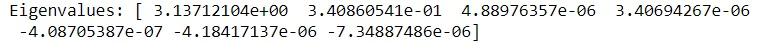
\includegraphics[width=0.5\textwidth]{Eigenvalues.jpg}
\end{figure}

\subsection{Initializing Newton's method with the solution of convex relaxation}

We can utilize the optimal solution $u^*$ obtained by solving \eqref{P''} using $\mathtt{cvxpy}$ to initialize Newton's method. Specifically, we can set $[x,y] = u^*$ as the starting point for Newton's method. This approach is implemented in our code without backtracking, and the resulting plot is \autoref{initialN}.

\begin{figure}[htbp]
    \centering
    \begin{subfigure}[b]{0.4\textwidth}
    \includesvg[width=\textwidth]{convergence_initconvex.svg}
    \caption{Convergence}
    \end{subfigure}
    \hfill
    \begin{subfigure}[b]{0.4\textwidth}  
    \includesvg[width=\textwidth]{chain_initconvex.svg}
    \caption{Chain solution}
    \end{subfigure}
    \caption{Initializing the Newton's method without backtracking with the solutions from \eqref{P''}}
    \label{initialN}
\end{figure}

In this specific instance, it appears that the Newton's method with the initial point set to $u^*$ converged in just one iteration. However, for other values of $N$, more iterations may be required. The convergence rate of Newton's method depends on various factors such as the initial guess, the conditioning of the problem, and the choice of step size.

We can compare the convergence of the three cases studied:
\begin{figure}[H]
    \centering
    \begin{subfigure}[b]{0.4\textwidth}
    \includesvg[width=\textwidth]{convergence_total.svg}
    
    \caption{Convergence for N=5}
    \end{subfigure}
    \hfill
    \begin{subfigure}[b]{0.4\textwidth}  
    \includesvg[width=\textwidth]{convergence_total_25.svg}
    \caption{Convergence for N=25}
    \end{subfigure}
    \caption{Convergence of Newton's method in the three cases studied.}
\end{figure}

\iffalse
Initializing Newton's method with the solution of convex relaxation problem, the algorithm converges fast towards a good solution, much more efficiently than using the original initialization proposed, which sometimes did not even converge without using backtracking. As this way we achieve a significantly faster and easier convergence, we can solve more complicated problems without such a high computational effort.
\fi
Utilizing the solution from the convex relaxation problem as an initialization for Newton's method can lead to expedited and more efficient convergence towards a favorable solution, as compared to a random initialization. This approach can also aid in guaranteeing that the algorithm converges to a viable solution, which may not be the case with a random initialization.

Moreover, by employing this technique, it is possible to address more intricate problems without incurring a significant computational cost, as the convergence is more rapid and dependable. This is especially useful in situations where the problem is computationally intensive, or where multiple instances of the problem need to be solved.

All in all, initializing Newton's method with the solution from the convex relaxation problem represents a promising method for tackling non-convex optimization problems efficiently and dependably.
\end{document}

